\renewcommand{\thechapter}{HS}
\chapter*{Homework Solutions}
\addtocounter{chapter}{1} % Manually increment the chapter counter
\markboth{\sffamily\normalsize\bfseries Homework Solutions}{} % Set the chapter header
\addcontentsline{toc}{chapter}{\textcolor{ocre}{Homework Solutions}}
\setcounter{section}{0}
\vspace{-0.3in}
\begin{tcolorbox}
    I encourage you to give each of the homework sets an honest attempt before looking at the solutions, you will get much more out of reading the solutions if you have first spent time carefully thinking about the problems on your own!
\end{tcolorbox}
\vspace{-0.2in}
\section{Homework \#1 Solutions}

\begin{enumerate}
    \item We are given the relation $\sim$ on $\R$:  
          \[
          \forall \ r,s \in \R, \quad r \sim s \iff r - s \in \Z
          \]
          and we are to show that $\sim$ is an equivalence relation.

          \textit{Proof:}  
          \begin{enumerate}
              \item \textbf{Reflexivity:} Take $r \in \R$. Then $r - r = 0$, and $0$ is an integer, so $r \sim r$.
              \item \textbf{Symmetry:} Assume $r \sim s$. Then $r - s$ is an integer.  
              Its ``opposite'' $-(r - s)$ is also an integer, so $s - r \in \Z$ and we have $s \sim r$.
              \item \textbf{Transitivity:} Assume $r \sim s$ and $s \sim t$.  
              Then $r - s \in \Z$ and $s - t \in \Z$. The sum of two integers is again an integer, so  
              \[
              (r - s) + (s - t) \in \Z
              \]
              so $r - t \in \Z$, so $r \sim t$. $\blacksquare$
          \end{enumerate}

    \item \begin{enumerate}
              \item The equivalence class of $\pi$ is given by:
                    \[
                    \text{cl}(\pi) = \{ r \in \R \mid r \sim \pi \}
                    \]
                    which means:
                    \begin{align*}
                        \text{cl}(\pi) &= \{ r \in \R \mid r - \pi \text{ is an integer} \} \\
                        &= \{ r \in \R \mid r = ( \text{an integer} ) + \pi \} \\
                        &= \{ n + \pi \mid n \in \Z \} = \{ \dots, -1+\pi, \pi, 1+\pi, 2+\pi, \dots \}
                    \end{align*}
                    This is usually expressed as $\pi + \Z$.
                    \begin{center}
                        \hspace{-0.1in}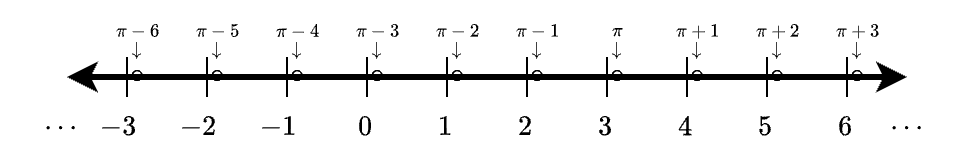
\includegraphics[width=0.85\textwidth]{Figures/EquivClassOfPiNumberLine.png}
                    \end{center}

              \item For any $s \in \R$, we can similarly find $\text{cl}(s)$ by substituting $s$ for $\pi$, so:
                    \[
                    \text{cl}(s) = s + \Z.
                    \]
                    Note that $\text{cl}(0)$ and $\text{cl}(1)$ are identical; they are both $\Z$.  
                    However, there are infinitely many $s \in \R$ between $0$ and $1$, and each such $s$ represents a class: $s + \Z$.  
                    So under the equivalence relation $\sim$ in problem (1), $\R$ is broken into infinitely many equivalence classes.
          \end{enumerate}
\end{enumerate}
% Problems 3-6
\begin{enumerate}
    \setcounter{enumi}{2}
    \item The following is an equivalence relation:  
          \[
          \forall n,m \in \Z, \quad n \sim m \iff n + m \text{ is even}.
          \]
          \textit{Proof:}  
          \begin{enumerate}
              \item \textbf{Reflexivity:} Take $n \in \Z$. Then $\underset{\substack{\ \ \ \ \ \ \ \ \ \ \ \ \ \ \ \uparrow \\ \ \ \ \ \ \ \text{the }``k" \text{ from defn. } \\
              \ \ \ \ \ \ \text{of ``even''}}}{n + n = 2n}$, which is even, so $n \sim n$.
              \item \textbf{Symmetry:} Assume $n \sim m$. Then $n + m$ is even, so there exists some $k \in \Z$ such that $n + m = 2k$.  
              Since addition in $\Z$ is commutative (i.e. $n+m=m+n$), we have $m + n = 2k$, which shows $m + n$ is even. Thus, $m \sim n$.
              \item \textbf{Transitivity:} Assume $n \sim m$ and $m \sim p$.  
              Then $\exists \ k \in \Z \ni $ $n + m = 2k$, and $\exists \ l \in \Z \ni $$m + p = 2l$.  
              Now,
              \[
              n + p = (2k - m) + (2l - m) = 2(k - m + l).
              \]
              Since $k, m, l$ are integers, $(k-m+l)$ is an integer, so $n+p$ is even, and $n \sim p$. $\blacksquare$
          \end{enumerate}

    \item Take $n \in \Z$; $n$ is either even or odd.  
          \begin{itemize}
              \item If $n$ is even, then $n + m$ is even $\iff m$ is even.  
              Since any even integer can be used for $m$, we have:
              \[
              \text{cl}(\text{any even } n) = 2\Z, \quad \text{the even integers.}
              \]
              \item If $n$ is odd, then $n + m$ is even $\iff m$ is odd.  
              This makes:
              \[
              \text{cl}(\text{any odd } n) = 1 + 2\Z, \quad \text{the odd integers.}
              \]
          \end{itemize}
          So the relation $\sim$ in (3) breaks $\Z$ into two classes: $2\Z$ and $1 + 2\Z$.

    \item Given $\sigma: \mathbb{R} \to \mathbb{Z}$ where $\sigma(r)$ is the smallest integer greater than or equal to $r$.  
          \[
          \sigma \text{ is not a bijection because it is not injective:}
          \]
          \[
          \frac{1}{2} \neq \frac{3}{4}, \text{ but } \sigma\left(\frac{1}{2}\right) = \sigma\left(\frac{3}{4}\right) = 1.
          \]

    \item Given $\alpha, \beta, \gamma: S \to S$ with $\gamma$ bijective, prove that $\alpha \circ \gamma = \beta \circ \gamma \implies \alpha = \beta$.  \\
          \textit{Proof:}  
          
              Since $\gamma$ is bijective, by L 1.2.3 $\exists$ $\gamma^{-1}: S \to S \ \ni \ \gamma \circ \gamma^{-1} = \gamma^{-1} \circ \gamma = I_S$. \\
              By hypothesis, $\alpha \circ \gamma = \beta \circ \gamma$ ; \ 
              Compose both sides with $\gamma^{-1}$ on the right:
                    \[
                    (\alpha \circ \gamma) \circ \gamma^{-1} = (\beta \circ \gamma) \circ \gamma^{-1}.
                    \]
              By associativity of composition (L 1.2.1) we can shift brackets:
              \begin{align*}
                &\alpha \circ (\gamma \circ \gamma^{-1}) = \beta \circ (\gamma \circ \gamma^{-1}). &\\
                \iff &\alpha \circ I_S = \beta \circ I_S & (\text{since }\gamma \circ \gamma^{-1} = I_S) \\
                \iff &\alpha = \beta. \ \ \ \ \ \blacksquare &
              \end{align*}
                    
              (For the last step, note that $\forall \ s\in S, (\alpha \circ I_S)(s) = \alpha[I_S(s)]=\alpha(s)$, so $\alpha \circ I_s = \alpha$. Likewise, $\beta \circ I_s =\beta$.)
          
\end{enumerate}


\newpage

\begin{tcolorbox}
    I encourage you to give each of the homework sets an honest attempt before looking at the solutions, you will get much more out of reading the solutions if you have first spent time carefully thinking about the problems on your own!
\end{tcolorbox}
\vspace{-0.2in}
\section{Homework \#2 Solutions}
\begin{enumerate}
    \item Compute $GCD(a, b)$ using the Euclidean algorithm:
          \begin{align*}
              138,000 &= 1 \cdot 102,810 + 35,190 \\
              102,810 &= 2 \cdot 35,190 + 32,430 \\
              35,190 &= 1 \cdot 32,430 + 2,760 \\
              32,430 &= 11 \cdot 2,760 + 2,070 \\
              2,760 &= 1 \cdot 2,070 + 690 \\
              2,070 &= 3 \cdot 690 + 0 \ \leftarrow \text{DONE;}
          \end{align*}
          Since the remainder is now $0$, $GCD$ is the last non-zero remainder: $GCD(a, b) = 690.$


    \item To express $GCD(a, b)$ as a linear combination:
    
    Throw away last equation; stack matrices $L\rightarrow R$ with quotients bottom to top; form in $\begin{bmatrix} 0 & 1 \\ 1 & -q \end{bmatrix}$
          \[
          \underset{\substack{5^{th} q \nearrow  }}{\begin{bmatrix} 0 & 1 \\ 1 & -1 \end{bmatrix}}
          \underset{\substack{4^{th} q \nearrow  }}{\begin{bmatrix} 0 & 1 \\ 1 & -11 \end{bmatrix}}
          \underset{\substack{3^{rd} q \nearrow  }}{\begin{bmatrix} 0 & 1 \\ 1 & -1 \end{bmatrix}}
          \underset{\substack{2^{nd} q \nearrow  }}{\begin{bmatrix} 0 & 1 \\ 1 & -2 \end{bmatrix}}
          \underset{\substack{1^{st} q \nearrow  }}{\begin{bmatrix} 0 & 1 \\ 1 & -1 \end{bmatrix}}
          = 
          \begin{bmatrix} * & * \\ 38 & -51 \end{bmatrix}
          \]
          Thus, we express $GCD(a, b)$ as:
          \[
          GCD(a, b) = 38a - 51b.
          \]
          So $n = 38$, $m = -51$.

    \item Given: $a, b, c \in \Z$, with $GCD(a, b) = 1$ and $GCD(a, c) = 1$.\\
    Prove: $GCD(a, bc) = 1$.\\

          \textit{Proof:}  
          \begin{align*}
            \text{By Lemma 1.3.1, since } &GCD(a, b) = 1 \implies \exists \ s, t \in \Z \ni \ 1=sa+tb \\
          \text{Similarly, since } &GCD(a, c) = 1 \implies \exists \ n, m \in \Z \ni \ 1 = na + mc.
          \end{align*}
          Now we can get $1$ as a linear combination of $a$ and $bc$:
          \begin{align*}
            1 = 1\cdot 1 = (sa+tb)(na+mc) &= sana + samc +tbna +tbmc \\
            &= \underbrace{(san + smc + tbn)}_{\in \Z}a + \underbrace{(tm)}_{\in \Z}bc
          \end{align*}
          The $GCD(a,bc)$ exists by Lemma 1.3.1; let's say it is $d$. \\
          Then $d|a$ and $d|bc$, so by Observation \#4 about divisions $d|(\substack{\text{linear combination} \\ \text{we found above}})$
          Since the linear combination equals $1$, we have $d|1$, so by Observation \#1 about divisions, $d=\pm 1$, but $GCD$ is defined as a \textit{positive} integer, so $d$ must be $1$. \\
          $\therefore \ \ GCD(a,bc)=1$. $\blacksquare$
          \newpage 
    \item Given $n, m, a \in \Z$, with $GCD(n, m) = 1$, and $n \mid a$ and $m \mid a$, \\
    Prove: $nm \mid a$. (so must express $a$ as an integer times $nm$) \\

          \noindent \textit{Proof:}  
          \begin{align*}
            \text{First, } &n \mid a \implies \ \exists \ k \in \Z \ni \ a = kn.  & \\
            & m \mid a \implies \ \exists \ l \in \Z \ni \ a = l m  & (\text{by defn of ``divides''})
          \end{align*}
          $GCD(n, m) = 1 \underset{L 1.3.1}{\implies} \ \exists \ x, y \in \Z \ni 1 = xn+ym$ \\
          Multiply this last equation by $a$:
          \begin{align*}
            a = a(xn + ym) = \underset{\substack{\uparrow \ \ \ \ \ \ \ \ \ \uparrow \ \ \ \ \\ a=lm \ \ \ \ \ \ \ \ \ a=kn \ \ \ \ }}{axn+aym} &= (lm)xn + (kn)ym \\ 
            &= \underbrace{(lx+ky)}_{\in \Z}nm
          \end{align*}
          $\therefore \ \ nm | a$. \ \ \ $\blacksquare$
\end{enumerate}

\begin{enumerate}
    \setcounter{enumi}{4} % Continue from previous numbering

    \item Given: $GCD(a, n) = 1$, and $\Z$ is partitioned by $\equiv \mod n$.  \\
          Prove: If $b \in [a]$, then $GCD(b, n) = 1$. \\

          \textit{Proof:}  
          Take $b \in [a]$. Then $b \equiv a \mod{n}$, so $n \mid (b - a)$, that is:
          \[
          \exists \ k \in \Z \ni b - a = kn.
          \]
          We also have $GCD(a, n) = 1$, so by Lemma 1.3.1, $\exists \ x, y \in \Z \ni 1 = xa + yn.$ \\
          We know $GCD(b, n)$ exists; let's call it $d$. [Idea: If I can get $1$ as a linear combination of $b$ and $n$, then it can be finished off like the end of the problem (3) proof]. 
          \begin{align*}
            1 = xa+yn \underset{\substack{\uparrow \\ b-a=kn \\ \text{so }a=b-kn}}{=} x(b-kn)+yn &= xb-wkn+yn \\
            &= \underset{\substack{\uparrow \\ \in \Z}}{x}b+ \underbrace{(y-xk)}_{\in \Z}n
          \end{align*}
          Now $d|b$ and $d|n$, so $d| \underbrace{\overset{\substack{lin. comb.}}{xb+(y-xk)n}}_{1}$ \ \ (again, by Observation \#4 about divisions [Prop 1.3.1 part 4]). \\
          Since $d|1$ and $d$ is a positive integer (it's a GCD), we must have $d = 1$. So $b$ and $n$ are relatively prime. Since $b$ was an arbitrary element of $[a]$, every element in $[a]$ is relatively prime to $n$. $\blacksquare$

    \item There are 4 possible Cayley tables for a group of order $4$, and each is symmetric across the main diagonal, proving that \textbf{every group of order 4 is abelian}.

    \begin{center}
        \begin{minipage}{0.45\textwidth}
            \centering
            \[
            \begin{array}{c||cccc}
                \cdot & e & a & b & c \\
                \hline \hline
                e & e & a & b & c \\
                a & a & b & c & e \\
                b & b & c & e & a \\
                c & c & e & a & b
            \end{array}
            \]
            If $a \cdot a = b$, you obtain this table.
        \end{minipage}
        \hfill
        \begin{minipage}{0.45\textwidth}
            \centering
            \[
            \begin{array}{c||cccc}
                \cdot & e & a & b & c \\
                \hline \hline
                e & e & a & b & c \\
                a & a & c & e & b \\
                b & b & e & c & a \\
                c & c & b & a & e
            \end{array}
            \]
            If $a \cdot a = c$, you obtain this one.
        \end{minipage}
    \end{center}

    \begin{center}
        \begin{minipage}{0.45\textwidth}
            \centering
            \[
            \begin{array}{c||cccc}
                \cdot & e & a & b & c \\
                \hline \hline
                e & e & a & b & c \\
                a & a & e & c & b \\
                b & b & c & a & e \\
                c & c & b & e & a
            \end{array}
            \]
            If $a \cdot a = e$, then you obtain either:\\
            i) This table, with $b \cdot b = a$.
        \end{minipage}
        \hfill
        \begin{minipage}{0.45\textwidth}
            \centering
            \[
            \begin{array}{c||cccc}
                \cdot & e & a & b & c \\
                \hline \hline
                e & e & a & b & c \\
                a & a & e & c & b \\
                b & b & c & e & a \\
                c & c & b & a & e
            \end{array}
            \]
            ii) Or this table, with $b \cdot b = e$.
        \end{minipage}
    \end{center}

    Since all possible Cayley tables are symmetric, every group of order $4$ is abelian.
\end{enumerate}

\newpage
\begin{tcolorbox}
    I encourage you to give each of the homework sets an honest attempt before looking at the solutions, you will get much more out of reading the solutions if you have first spent time carefully thinking about the problems on your own!
\end{tcolorbox}
\vspace{-0.2in}
\section{Homework \#3 Solutions}